
\section{Multi-way Merge Semantic \textsf{ORDER BY}}

% \begin{table}[t]
% \footnotesize
%   \caption{Frequently-used notations throughout the paper}
%   \label{tab:params}
%   \footnotesize
%   \centering
%   \begin{tabular}{@{}cl@{}}
%     \toprule
%     \textbf{Notation} & \textbf{Description} \\
%     \midrule
%     $D$ & Input item collection \\
%     $n$ & Input size ($n=|D|$) \\
%     $\phi$ & Natural-language ordering instruction \\
%     $m$ & Maximum items per listwise call \\
%     $K$ & Requested prefix length \\
%     $\Pi$, $\Pi_K$ & Full order and top-$K$ prefix \\
%     $k$ & Maximum merge fan-in \\
%     $r$ & Initial run count ($r=\lceil n/m \rceil$) \\
%     $h$ & Per-run window or segment quota \\
%  %   $C$ & Total number of listwise calls \\
%     \bottomrule
%   \end{tabular}
% \end{table}

We introduce our algorithmic overview of $k$-way merge semantic \textsf{ORDER BY}, where listwise LLM calls $\textsc{ListwiseRank}(\cdot,\phi)$ over batches of at most $m$ items are the only ranking primitives.
Algorithm~\ref{alg:semantic_external_merge} shows the procedure of the $k$-way merge, which consists of two phases: run generation and iterative $k$-way merge. 


\stitle{Phase 1: run generation.} Lines 1–6 construct the initial sorted runs. The algorithm first assigns each item a temporary identifier, which is used to track item provenance across LLM calls and to validate the model output (line 1). The input collection $D$ is then partitioned into $r=\lceil |D|/m \rceil$ chunks, each containing at most $m$ items (line 2). Each chunk is independently ranked under the instruction $\phi$ using one listwise call (line 4-5).
Since the chunks are disjoint, these calls can be issued in parallel. The resulting $r$ locally sorted sequences are collected as the initial run list $\mathcal{L}$ (line 6).

% \emph{Phase 1 (lines 1--6): run generation.}
% Line~2 assigns every item a temporary identifier. The identifier lets
% the merger track item provenance across listwise calls and detect
% items that the model drops, duplicates, or fabricates in its output;
% the identifiers are stripped before the final result is returned
% (line~16). Line~3 partitions the input $D$ into
% $r=\lceil |D|/m \rceil$ chunks of at most $m$ items, the largest unit
% a single listwise prompt can hold. Lines~4--5 sort each chunk under
% the instruction $\phi$ with one listwise call per chunk; the calls
% are mutually independent and issued in parallel. Line~6 collects the
% $r$ sorted runs into the working list $\mathcal{L}$.

\stitle{Phase 2:  iterative $k$-way group merge.} Lines 7–15 repeatedly merge the current run population until only one run remains. Each loop iteration corresponds to one merge pass. At the beginning, a cost model computes an optimal fan-in $k$ based on the number of items $|D|$, the listwise batch size $m$, and the chosen group-merging implementation of $\textsc{MergeGroup}$. We defer the instantiations of $\textsc{MergeGroup}$ by a sliding window $k$-way merge or loser-tree $k$-way merge in \cref{sec:sw} and \cref{sec:lt}, respectively.
In one merge pass, the algorithm first partitions the current runs $\mathcal{L}$ into $s=\lceil |\mathcal{L}|/k \rceil$ groups, each containing at most $k$ runs (line 11). Each group is merged into a single sorted run by the $k$-way merge algorithm $\textsc{MergeGroup}$ (lines 12-14).
Groups within the same pass are independent, so the merge operations in a pass can also be executed in parallel.
After all groups have been merged, the newly produced runs replace $\mathcal{L}$ (line 15), reducing the number of runs by approximately a factor of $k$. The process terminates when $\mathcal{L}$ contains a single run; the temporary identifiers are then stripped, and the resulting sequence is returned as the final semantic order (lines 16-17).


% \emph{Phase 2 (lines 7--15): iterative $k$-way merging.}
% Each iteration of the loop performs one merge pass. Line~9 invokes
% the cost model to select the fan-in $k$ for the
% current pass from the surviving run population $|\mathcal{L}|$, the
% batch size $m$, and the group merger in use. The two mergers have
% different cost profiles, and the effective fan-in of the final pass
% can be smaller than that of earlier passes, so $k$ is chosen per pass
% rather than fixed once. Line~11 partitions $\mathcal{L}$ into
% $s=\lceil |\mathcal{L}|/k \rceil$ groups of at most $k$ runs each.
% Lines~12--14 merge every group into a single sorted run through the
% plug-in $\textsc{MergeGroup}$, instantiated by the sliding-window
% merger (Algorithm~\ref{alg:sliding_window_kway_group_merge}) or the loser-tree merger (Algorithm~\ref{alg:loser_tree_kway_group_merge}); groups
% are independent, so each pass parallelizes across groups. Line~15
% replaces the run population with the merged runs, shrinking it by a
% factor of roughly $k$. The loop terminates when a single run remains;
% line~16 removes the temporary identifiers and returns it.

In the following, we present an example for Algorithm~\ref{alg:semantic_external_merge}, followed by our instantiated $k$-way merge algorithms using sliding window and a loser tree, respectively. Each algorithm, based on its implementation, adopts a token cost model to select the optimal fan-in $k$, expecting to achieve a minimum token cost (\cref{sec:cost})
%. \cref{sec:cost} will introduce the cost models.



\begin{algorithm}[t]
\small
\caption{External Merge Group via $k$-Way Merge}
\label{alg:semantic_external_merge}
\KwIn{Dataset $D$, listwise batch size $m$, semantic instruction $\phi$, group merger $\textsc{MergeGroup}()$}
\KwOut{final semantic sorted run $\Pi$}

\textbf{Phase 1: Run generation} \;
Assign every item a temporary id \;
Partition $D$ into chunks $\mathcal{C}_1,\dots,\mathcal{C}_r$ of size at most $m$ \;
\For{$i \gets 1$ \KwTo $r$ \textbf{in parallel}}{
    $R_i \gets \textsc{ListwiseRank}(\mathcal{C}_i,\phi)$ \;
}
$\mathcal{L} \gets [R_1,\dots,R_r]$ \;

\textbf{Phase 2: Iterative $k$-way group merging} \;
$k \gets \textsc{MergeCostModel}(|D|, m, \textsc{MergeGroup})$ \algocomment{choose merge fan-in automatically for this round} \;
\While{$|\mathcal{L}| > 1$}{
    $\mathcal{L}_{next} \gets [\ ]$ \;
    Partition $\mathcal{L}$ into groups $\mathcal{G}_1,\dots,\mathcal{G}_s$ with at most $k$ runs each \;
    \For{$j \gets 1$ \KwTo $s$ \textbf{in parallel}}{
        $Q_j \gets \textsc{MergeGroup}(\mathcal{G}_j,\phi,k)$ \;
        Append $Q_j$ to $\mathcal{L}_{next}$ \;
    }
    $\mathcal{L} \gets \mathcal{L}_{next}$ \;
}
$\Pi \gets \mathcal{L}[1]$, Remove temporary ids from $\Pi$ \;
\Return{$\Pi$} \;
\end{algorithm}


\begin{figure}[t]
    \centering
    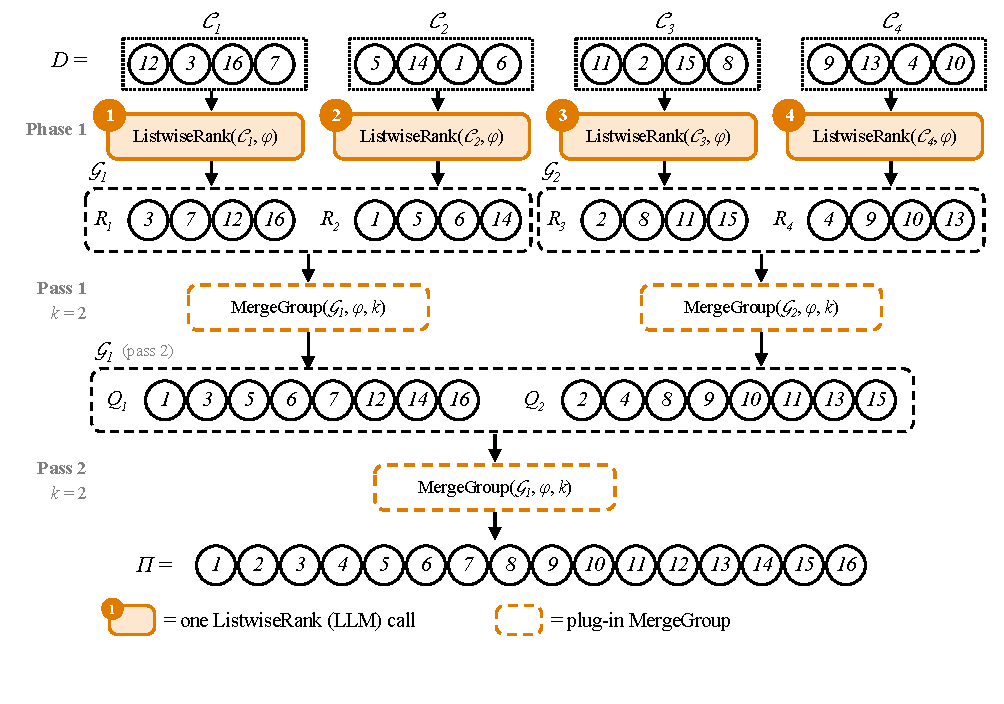
\includegraphics[width=0.95\linewidth]{fig/algo1-exp.pdf}
    \caption{Example of Algorithm~\ref{alg:semantic_external_merge}: 4 runs generation, then two merge passes.}
    \label{fig:exp:semantic_external_merge}
\end{figure}

\begin{example}\label{ex:alg1}
Fig~\ref{fig:exp:semantic_external_merge} traces Algorithm~\ref{alg:semantic_external_merge} on $n=16$ items with batch size $m=4$.
Phase~1 partitions $D$ into $r=\lceil 16/4\rceil=4$ chunks and sorts
each chunk with one listwise call, yielding 4 runs
$R_1$, $R_2$,
$R_3$, and $R_4$
(line~1--6). Phase~2 starts from $|\mathcal{L}|=4$; Suppose
\textsc{MergeCostModel} selects fan-in $k=2$ (line 7), therefore the sorting takes $\lceil\log_2 4\rceil=2$ merge passes. 
Pass~1
partitions $\mathcal{L}$ into $s=2$ groups,
$\mathcal{G}_1=\{R_1,R_2\}$ and $\mathcal{G}_2=\{R_3,R_4\}$, and merges
the groups in parallel through the \textsc{MergeGroup},
producing $Q_1$ and
$Q_2$ (lines~11--15). Pass~2 finally merges
$\{Q_1,Q_2\}$ into $\Pi=[1,\dots,16]$.
\end{example}



% \begin{example}\label{ex:alg1}
% Fig~\ref{fig:exp:semantic_external_merge} traces Algorithm~\ref{alg:semantic_external_merge} on $n=16$ items with batch size $m=4$.
% Phase~1 partitions $D$ into $r=\lceil 16/4\rceil=4$ chunks and sorts
% each chunk with one listwise call, yielding 4 runs
% $R_1=\langle 3,7,12,16\rangle$, $R_2=\langle 1,5,9,14\rangle$,
% $R_3=\langle 2,8,11,15\rangle$, and $R_4=\langle 4,6,10,13\rangle$
% (lines~3--6). Phase~2 starts from $|\mathcal{L}|=4$;
% \textsc{MergeCostModel} selects fan-in $k=2$ (line~9). Pass~1
% partitions $\mathcal{L}$ into $s=2$ groups,
% $\mathcal{G}_1=\{R_1,R_2\}$ and $\mathcal{G}_2=\{R_3,R_4\}$, and merges
% the groups in parallel through the plug-in \textsc{MergeGroup},
% producing $Q_1=\langle 1,3,5,7,9,12,14,16\rangle$ and
% $Q_2=\langle 2,4,6,8,10,11,13,15\rangle$ (lines~11--15). Pass~2 merges
% $\{Q_1,Q_2\}$ into $\Pi=\langle 1,\dots,16\rangle$, and line~16 strips
% the temporary identifiers. The schedule takes
% $\lceil\log_2 4\rceil=2$ passes; each numbered circle in the figure is
% one listwise call, and each dashed box is one \textsc{MergeGroup} algorithm 
% instance.
% \end{example}

\section{Sliding Window Multi-way Merge}
\label{sec:sw}

We propose a sliding window $k$-way merge algorithm as an instantiation of $\textsc{MergeGroup}$. The algorithm is an adaptation to listwise ranking from classical external $k$-way merge sort~\cite{DBLP:journals/csur/Graefe06}. 
In classical external $k$-way merge, the algorithm iteratively compares the current heads of the input runs and emits the smallest one. The ordering of the input runs is sufficient to guarantee that the emitted item is globally next.
For semantic \textsf{ORDER BY}, considering $\textsc{ListwiseRank}$ is the only available comparison primitive with a nontrivial cost, a direct head-by-head adaptation would therefore require one LLM call per emitted item.
To improve the throughput of $\textsc{ListwiseRank}$ regarding item emission, Algorithm~\ref{alg:sliding_window_kway_group_merge} packs head items from \emph{each} active run, so that a single call ranks up to $m$ candidate items across the group. In one $\textsc{ListwiseRank}$ call, since the LLM ranker can see only head items of the runs, its complete ranking output may not be globally ordered. The algorithm identifies a `safe prefix' from the output (line~18--22), and only emits this prefix. 



% Algorithm~2 merges a group of $k$ sorted runs by repeatedly ranking a
% window drawn evenly from all runs and emitting only the prefix of the
% ranking that can be certified as globally correct.

% The algorithm is the listwise counterpart of the $k$-way merge step of
% classical external merge sort~\cite{DBLP:journals/csur/Graefe06}. The
% classical merger repeatedly emits the smallest current run head: every
% decision is one exact two-item comparison, essentially free on a CPU,
% and the sortedness of the runs alone certifies each emission. Under a
% semantic order the only comparison primitive is a listwise call that
% ranks up to $m$ items at a fixed per-call price, so a head-by-head
% port would spend one call per emitted item. Algorithm~2 adapts the
% merge to this primitive: it packs items from \emph{all} active runs
% into one call, so a single call settles the relative order of up to
% $m$ items drawn across the group, and the certified-prefix rule
% (lines~18--22) restores the correctness argument that sortedness no
% longer provides, since the ranker sees only a bounded window of each
% run. The design also departs from the two-way external merge of prior
% LLM-based sorting~\cite{DBLP:journals/corr/abs-2509-00303}, which is
% in effect the $k=2$ instance of this scheme: hard-wiring the fan-in to
% two commits every schedule to $\lceil\log_2 r\rceil$ passes over $r$
% Phase-1 runs---the maximum over all feasible fan-ins---with every pass
% re-ranking the entire input. Algorithm~2 instead keeps the fan-in a
% free parameter, sound for any $g \ge 2$, and defers its choice to the
% cost model of \cref{sec:sw-cost}.

Algorithm~\ref{alg:sliding_window_kway_group_merge} maintains a read cursor $p_i$ for each run and an output sequence $\Pi$ (line 1). Each round of the loop (lines~3--24) issues one listwise call and emits a safe prefix of the LLM output. At the start of a round, line 3 identifies the active runs 
$A$, namely those with unread items.  If no active runs remain, the merge is complete (lines 4-5). If only one run remains active, lines 6–9 append its unread suffix directly to $\Pi$ without an LLM call, because it is already sorted. 
When more than one run remains active, line 10 divides the prompt budget evenly across them. Each active run receives a quota of $h=\lfloor m/|A| \rfloor$ items to be sorted by a $\textsc{ListwiseRank}$ call. 
Lines 11–16 assemble the batch $B$, where each active run $R_i$ contributes its next $b_i \leq h $ unread items, denoted as $W_i$. 
The algorithm also initializes a counter $e_i$  for each active run (line 15), recording how many contributed items from that run are emitted in the current round.
Line 17 invokes $\textsc{ListwiseRank}(B,\phi)$, producing a ranked order $\mathcal{O}$ over the batch. 
Lines~18--22 emit only the safe prefix of $\mathcal{O}$. The algorithm scans $\mathcal{O}$ in rank order,  appending each item to $\Pi$ and increasing the emitted counter $e_i$ of its  originating run. The scan stops once some run $R_t$ has had its contributed window fully emitted ($e_t=b_t$, lines~21--22).
This stopping criterion for emitting is required to ensure global orderedness: 
Once $W_t$ emits, the next unseen item from $R_t$ is not included in the current LLM call; it may therefore precede every remaining item in $\mathcal{O}$ under the semantic instruction $\phi$. Consequently, no item ranked after this point is safe as the next global output. 
Lines 23–24 then advance each cursor $p_i$ by exactly $e_i$ items emitted from that run. Any un-emitted suffix of $\mathcal{O}$ is processed again in the next call, where it competes against new arrival items from active runs. When all runs have been consumed, line 25 returns the merged sequence.

This algorithm is a generalization of the two-way external merge for LLM-based sorting~\cite{DBLP:journals/corr/abs-2509-00303}, which corresponds to the special case $k=2$. Fixing $k=2$ forces the merge schedule to use $\lceil\log_2 r\rceil$ passes over $r$ runs from Phase 1 of Algorithm~\ref{alg:semantic_external_merge}. 
In contrast, Algorithm~\ref{alg:sliding_window_kway_group_merge} emits $h$ items in the worst case, and $(h-1)|A|+1 \leq m-|A|+1$ in the best case. 
There exists an optimal fan-in $k$ in $\{2,\ldots, \lfloor m/2\rfloor\}$ maximizing expected item throughput of listwise calls (\cref{sec:cost}), where the upper bound ensures that each active run contributes at least two items and each listwise possibly emits more than one item. 

%, where the upper bound ensures that each active run contributes at least two items to a full window.

% Line~1 initializes a read cursor $p_i$ for every run and an empty
% output $\Pi$. Each iteration of the loop (lines~2--24) issues exactly
% one listwise call. Line~3 computes the set $A$ of active runs, those
% with unread items; lines~4--5 terminate when all runs are exhausted.
% Lines~6--9 handle the single-run case without any LLM call: when only
% one run remains active, its unread suffix is already sorted under
% $\phi$, because it was produced either by a Phase-1 listwise sort or
% by an earlier certified merge, so it is appended to $\Pi$ verbatim.

% Line~10 divides the window budget evenly among the active runs,
% giving each a quota of $h=\lfloor m/|A| \rfloor$ items so that the
% combined batch never exceeds the prompt capacity $m$. Lines~11--16
% assemble the batch $B$: every active run $i$ contributes the next up
% to $h$ unread items $W_i$ (fewer if the run is nearly exhausted); the
% counter $b_i$ records how many items run $i$ contributed and $e_i$
% counts how many of them are emitted in this round. Line~17 ranks the
% batch with one listwise call, yielding the order $\mathcal{O}$.

% Lines~18--22 emit the certified prefix of $\mathcal{O}$. The loop
% scans $\mathcal{O}$ in rank order, appends each item to $\Pi$, and
% credits its originating run; it stops as soon as some run $t$ has had
% its entire window emitted ($e_t=b_t$, lines~21--22). The stop is
% required for correctness rather than efficiency: once run $t$'s
% window is drained, the next unseen item of run $t$ may precede, under
% $\phi$, every remaining item in the batch, so no item ranked after
% this point can be certified as the global successor. Lines~23--24
% advance each cursor by exactly the emitted count $e_i$; the unemitted
% suffix of every window stays in place and re-enters the next batch,
% where it competes against fresh items from the previously exhausted
% run. Line~25 returns the merged run.

% Per listwise call, the emitted count therefore lies between $h$
% (worst case: the batch drains one window before emitting anything
% else) and $(h-1)|A|+1 = m-|A|+1$ (best case: every window retains one
% item when the first exhaustion occurs). 



\begin{algorithm}[t]
\small
\caption{Sliding-Window Semantic $k$-Way Merge}
\label{alg:sliding_window_kway_group_merge}
\KwIn{a group of sorted runs $\mathcal{G}=\{R_1,\dots,R_k\}$, instruction $\phi$, listwise batch size $m$}
\KwOut{one merged sorted run $\Pi$}

Initialize cursor $p_i \gets 0$ for every run $R_i$, $\Pi \gets [\ ]$ \;

\While{at least one run in $\mathcal{G}$ is not exhausted}{
    $A \gets \{R_i \mid p_i < |R_i|\}$ ; \algocomment{collect active runs} \\
    \If{$A=\emptyset$}{
        \textbf{break} \;
    }
    \If{$|A|=1$}{
        let $R_u$ be the only active run in $A$ \;
        Append $R_u[p_u:|R_u|]$ to $\Pi$ \;
        \textbf{break} \;
    }

    $h \gets \lfloor m / |A| \rfloor$ ; \algocomment{window size contributed by each active run} \\
    $B \gets [\ ]$ \;

    \ForEach{$R_i \in A$}{
        $W_i \gets$ up to $h$ items from $R_i[p_i:]$ \;
        $b_i \gets |W_i|$ ; \algocomment{items contributed by run $i$ in this batch} \\
        $e_i \gets 0$ ; \algocomment{items emitted from run $i$ in this batch} \\
        Append $W_i$ to $B$ \;
    }

    $\mathcal{O} \gets \textsc{ListwiseRank}(B,\phi)$ \;

    \ForEach{$x \in \mathcal{O}$}{
        let $R_t$ be the originating run of $x$ \;
        Append $x$ to $\Pi$, $e_t \gets e_t + 1$ \;
        \If{$e_t = b_t$ \textbf{and} $p_t + b_t < |R_t|$}{
            \textbf{break} ; \algocomment{run $R_t$ drained its window but still has unseen items} \\
        }
    }

\ForEach{$R_i \in A$}{
    $p_i \gets p_i + e_i$ ; \algocomment{update cursors; unsafe suffix of $\mathcal{O}$ stay pending} \;
}
}

\Return{$\Pi$}
\end{algorithm}

% Approved: PR9 cursor/sw-sliding-window-figure-ad37, recovery/sw/sw-wide.pdf
\begin{figure*}[t]
    \centering
    \includegraphics[width=\textwidth]{sw-wide.pdf}
    \caption{Example of Algorithm~\ref{alg:sliding_window_kway_group_merge} for sliding window merge $(m = 8, h = \lfloor m / |A|\rfloor)$: three calls emit $5+5+6=16$ items.
    \emph{Integration note:} synthetic layout placeholder for type-setting review; not a measured execution trace.}
    \label{fig:eg:sliding_window}
\end{figure*}

\begin{example}\label{ex:alg2}
Fig.~\ref{fig:eg:sliding_window} illustrates a sliding-window merge with $k = 4$ sorted runs and batch size $m = 8$. In Round 1, all runs are active, so each receives quota $h=\lfloor 8/4\rfloor=2$. The batch contains the first two unread items from each run, $B=\{3,7,1,5,2,8,4,9\}$. The listwise call returns $\mathcal{O} = [1, 2, 3, 4, 5, 7, 8, 9]$. The algorithm emits the safe prefix $[1, 2, 3, 4, 5]$ and stops when $R_2$'s window $[1, 5]$ is exhausted, because the unseen item $6$ from $R_2$ may precede the remaining ranked items. 
In Round 2, the unemitted items ${7, 8, 9}$ re-enter the batch together with new arrival items, forming a batch $B = \{7,12,6,14,8,11,9,10\}$. The The listwise call returns $\mathcal{O} = [6,7,8,9,10,11,12,14]$. The safe prefix $[6, 7, 8, 9, 10]$ is emitted and the scan stops $R_4$'s window $[9, 10]$ is exhausted. The process continues until full ranking $\Pi$ is generated over $k$ runs. 

% Algorithm~2 on the four Phase-1 runs of Figure~1 with
% $m=8$. In Round~1 all four runs are active, so each receives a quota
% $h=\lfloor 8/4\rfloor=2$ and contributes its next two items, giving
% $B=\{3,7,1,5,2,8,4,6\}$; one listwise call returns
% $\mathcal{O}=\langle 1,\dots,8\rangle$. The emission loop appends
% $1,2,3,4,5$ and then stops: run $R_2$ has had its entire window
% emitted ($e_2=b_2=2$) while it still holds unseen items, and the
% unseen item $9$ may precede $6,7,8$ under $\phi$, so $6,7,8$ cannot be
% certified and re-enter the next batch (lines~21--22). Round~2
% assembles $B=\{7,12,9,14,8,11,6,10\}$ and emits $6,\dots,10$, again
% truncated after five items when $R_4$'s window drains. In Round~3 the
% nearly exhausted runs contribute $b_2=b_4=1$, so $|B|=6$; every
% draining run is fully exhausted, no truncation applies, and all six
% items $11,\dots,16$ are emitted. Three calls emit $5+5+6=16$ items,
% between the per-call bounds $h$ and $m-|A|+1$ of Section~4.
\end{example}

\section{Loser Tree Multi-way Merge}
\label{sec:lt}

This section proposes algorithmic instantiations of $\textsc{MergeGroup}$ via tournament data structures, including two algorithms with a loser tree~(\cref{sec:lt:binary}) and an optimized segmented loser tree (\cref{sec:lt:segment}). 

\subsection{Loser Tree}
\label{sec:lt:binary}

Algorithm~\ref{alg:loser_tree_kway_group_merge} replaces the flat window of Algorithm~\ref{alg:sliding_window_kway_group_merge} 
with a loser tree over $k$ runs. 
Recall the classical loser tree used in external merge sort~\cite{DBLP:journals/csur/Graefe06}; the leaves correspond to the $k$ runs, and each internal node stores the loser of a match between two subtree winners, and the root stores the overall champion. 
When a leaf is updated, only the $O(\log k)$ matches on the path to the root should be recomputed. This order locality makes loser tree suitable for tournament-style LLM ranking. 
Algorithm~\ref{alg:loser_tree_kway_group_merge} adapts classical loser tree to listwise LLM ranking at two points. First, a loser tree is initialized by \textsc{InitLoserTree}, ranking $k$ run heads in a single listwise call. Second, leaf update triggers a \textsc{RefreshPath}, batching the updated run head together with the stored losers along the affected path and ranking this set in one listwise call.



% structure. A loser tree over $k$ runs maintains, after $O(\log k)$
% comparisons per update, the invariant that the root's current winner
% is the globally best unemitted item; a merge then reduces to
% repeatedly popping the root and repairing a single leaf-to-root path.


% The loser tree is the classical tournament structure of external merge
% sort~\cite{DBLP:journals/csur/Graefe06}: leaves hold the $k$
% contestants, each internal node remembers the loser of one match, the
% root holds the champion, and replacing a leaf re-plays only the
% matches on that leaf's bracket path, since every other recorded
% outcome is unaffected. Exactly this match locality makes the structure
% relevant to tournament-style LLM
% ranking~\cite{DBLP:journals/corr/abs-2603-17223}, in which the model
% acts as the judge of each match: the matches invalidated by one
% emission form a single short path, a closed candidate set of at most
% $1+\lceil\log_2 g\rceil$ items that fits comfortably into one prompt.
% The classical merger, however, plays the path as a chain of exact
% pairwise comparisons---free on a CPU, but one LLM call each under a
% semantic order, and inherently sequential because every match waits
% for the winner of the previous one. Algorithm~3 adapts the structure
% to the listwise primitive at both interaction points:
% \textsc{InitLoserTree} ranks the $k$ run heads in one call and replays
% the entire construction tournament through rank-map lookups in place
% of $g-1$ comparison calls, and \textsc{RefreshPath} batches the new
% representative together with the stored losers of the path into one
% listwise call whose local ranks settle all path matches at once. The
% tournament bookkeeping is inherited verbatim; only the comparison
% currency changes, and the price of a pop drops from
% $\lceil\log_2 g\rceil$ sequential decisions to exactly one call.

We explain the detailed procedure of Algorithm~\ref{alg:loser_tree_kway_group_merge}. Line 1 initializes the read cursors $p_i$, and line 2 forms the set of active runs $A$. 
Lines 3–4 handle the degenerate case in which all runs are empty. Lines 5–6 collect the head item of each active run, i.e., its current representative $x_i$. In line 7, the algorithm initializes the loser tree by $\textsc{InitLoserTree}$, and the output permutation $\Pi$. The main loop in lines 8–19 emits one item per round, triggering one listwise call in the procedure $\textsc{RefreshPath}$ for tree maintenance (line 19). 
Lines~9--12 address the corner case in which a single active run remains, similar to lines 6--9 in Algorithm~\ref{alg:sliding_window_kway_group_merge}. 
The algorithm pops the current winner $x_u$ from the root, which originally comes from run $R_u$ (line 13). Based on the order locality of loser tree, $x_u$ is the current highest-ranked representative and the next global output item. Line 14 therefore emits $x_u$ to $\Pi$ and advances the cursor of $R_u$. Lines 15-16 extract the new head item from $R_u$ as the new representative $x_u$ if $R_u$ is non-exhausted; otherwise, $R_u$ is deactivated (lines 17--18).
Finally, line 19 calls $\textsc{RefreshPath}$ to maintain the locality of the loser tree, which spends exactly one listwise call. We first briefly introduce the path refresh algorithm, $\textsc{RefreshPath}$, followed by tree construction, $\textsc{InitLoserTree}$.
 
% Line~1 initializes the cursors, and line~2 restricts attention to the
% set $A$ of non-empty runs; lines~3--4 dispose of the degenerate empty
% input. Lines~5--6 load the head of every active run as its current
% representative $X_i$. Line~7 builds the loser tree with
% $\textsc{InitLoserTree}$ (Algorithm~\ref{alg:init_loser_tree}) and initializes the output.

% The main loop (lines~8--19) emits one item per iteration.
% Lines~9--12 are the single-run fast path of Algorithm~2: the last
% surviving run's suffix is appended without further LLM calls.
% Line~13 reads the overall winner $u$ at the root, whose
% representative $X_u$ is the highest-ranked unemitted item under
% $\phi$. Line~14 emits $X_u$ and advances run $u$'s cursor.
% Lines~15--18 either promote run $u$'s next item to be its new
% representative or, if run $u$ is exhausted, remove $u$ from $A$ and
% deactivate its leaf. Line~19 restores the tree invariant with
% $\textsc{RefreshPath}$ (Algorithm~\ref{alg:refresh_loser_tree_path}). Only the nodes on the path from
% $\text{Leaf}(u)$ to the root can be affected by the change at leaf
% $u$, so each emission touches at most
% $\lceil \log_2 g \rceil$ internal nodes and, as shown below, costs
% exactly one listwise call.
\stitle{Tree construction:} 
$\textsc{InitLoserTree}$ constructs the initial loser tree over the representatives of the $k$ runs, at most, in one group. 
Listwise ranking computes the ranking of the $k$ representatives and returns a rank map $\rho$ for lookup. If $k \leq m$, one listwise call can accommodate these representatives; Otherwise, if $k > m$, we invoke two-way sliding window merge to process the ranking. Then, $\textsc{InitLoserTree}$ initializes a complete binary tree, padding empty leaves with \textsc{null} and replays the tournament bottom-up by looking up $\rho$ for pairwise item comparison. When both children are non-null, the child with the higher rank wins and  propagates upward. After all matches are replayed, the root stores the global winner of the current group. 


% e$\textsc{InitLoserTree}$ (Algorithm~\ref{alg:init_loser_tree}) constructs an initial loser tree over the representatives of the $g$ runs in the current group. Unlike classical tournament tree construction, which performs a pairwise comparison at every internal node, listwise ranking first obtains a global order over all resident candidates and then builds the loser tree  through rank-map lookups, avoiding an LLM call for each match. 

% Specifically, $\textsc{InitLoserTree}$ collects the $X_{\mathrm{init}}=\{x_i\mid i\in A\}$ resident representatives. If $|X_{\mathrm{init}}|\le m$, one listwise call ranks them. Otherwise, it ranks batches of at most $m$ items and repeatedly merges the two shortest resulting runs with the fan-in-two sliding-window merger. The final run $Q_{\mathrm{init}}$ defines the rank map $\rho$.

% The algorithm then seeds a complete binary loser tree, pads unused leaves with \textsc{null}, and replays the tournament bottom-up using $\rho$. A \textsc{null} child forwards the other candidate; otherwise, the winner propagates upward and the loser is stored at the node. The root stores the resulting global winner.

%Line~1 ranks these representatives with one listwise call, and 
%line~2 converts the returned order into a rank map $\rho$ as an index for subsequent lookup. 
%Line 3 allocates a complete binary tree, padding the empty leaves with \textsc{null}, and lines 3-7 seed the leaves with the representatives. Lines 8–18 then play the tournament bottom-up, where pairwise comparisons look up the index $\rho$. After construction, the root gives the current global winner in $O(1)$ time. 

% Line~1 ranks the $k$ representatives with a single listwise call, and
% line~2 converts the returned order into a rank map $\rho$. All
% comparisons during construction are then $\rho$-lookups, so building
% the tree issues no further LLM calls. Line~3 allocates a complete
% binary tree, padding the leaf level to a power of two with
% \textsf{null} leaves; lines~4--7 seed the leaf winners. Lines~8--18
% play the tournament bottom-up: at every internal node the two child
% winners are compared through $\rho$ (lines~15--18), the winner
% propagates upward, and the loser is stored at the node;
% \textsf{null} children simply forward the other child (lines~11--14).
% The resulting structure supports winner extraction in $O(1)$ and path refresh in $O(\log k)$.

% In steady state the merger thus pays one listwise call over
% $O(\log k)$ items per emitted element. \cref{sec:slt} introduces a segmented variant in which each leaf holds a segment of $h$ items and each refresh emits $h$ items per call; \cref{sec:lt-cost} models the call count of both variants and derives the optimal fan-in for each.
\stitle{Path refresh:}
$\textsc{RefreshPath}$ maintains loser tree orderedness after one representative of run $R_u$ updates. Unlike the maintenance of a classical loser tree, which scans the affected path once, path refresh with a listwise ranking sweeps the affected path twice: the first sweep collects the items to be ranked in one batch, and the second pass updates the path using the ranking output. 
Specifically, $\textsc{RefreshPath}$ first collects the batch $B$ to be ranked. This set contains the updated representative of run $R_u$ if $R_u$ is still active, together with the stored losers on the path from $\text{Leaf}(R_u)$ to the root. Losers belonging to exhausted runs are skipped. Since the path contains at most one stored loser per level, $|B| \le 1+\lceil \log_2 k \rceil$. Then, items in $B$ are sorted by a listwise call, and a rank map $\rho_{path}$ preserves the ranking.
The second sweep replays the standard tournament along the same path, where pairwise comparisons look up the index $\rho_{path}$.
%A variable $w$ stores the candidate currently propagating upward, initialized to the updated run $R_u$ or to \textsc{null} if $R_u$ has been exhausted (lines 16--19). In lines 20--33, along each ancestor node, $w$ is compared with the node’s stored loser $r$ using path $\rho_{path}$. The higher-ranked candidate continues upward, and the lower-ranked one becomes the node’s new stored loser. If either side is null because a run has been exhausted, the non-null candidate is forwarded. 
When the replay reaches the root, all affected matches have been repaired, and $\textsc{CurrentWinner}(T)$ will return the next global best.

% The procedure runs in two sweeps over the same path. The first sweep
% (lines~1--10) collects the comparison set $\mathcal{P}$: the updated leaf's new
% representative, if run $u$ is still active (lines~2--3), together
% with the stored losers along the path from $\text{Leaf}(u)$ to the
% root (lines~5--10), skipping losers whose runs are exhausted. Since
% the path holds one stored loser per level,
% $|P| \le 1+\lceil \log_2 g \rceil$. Lines~11--12 short-circuit when
% there is nothing to compare. Line~13 ranks $P$ with a single listwise call and line~14 builds the local rank map $\rho_{path}$; this is the only LLM interaction of the refresh. The second sweep (lines~15--33)
% replays the tournament along the path: $a$ holds the candidate
% propagating upward, initialized to $u$ or \textsf{null}
% (lines~16--19). At every ancestor, the candidate meets the stored
% loser $q$; the one ranked higher by $\rho_{path}$ continues upward
% while the other is stored as the node's new loser (lines~28--32), and
% the \textsf{null} cases arising from exhausted runs are resolved by
% forwarding whichever side remains (lines~23--27). When the sweep
% reaches the root, the invariant holds again and
% $\textsc{CurrentWinner}(T)$ is the next global head.

The loser tree maintains global orderedness for the current representatives of all active runs. This design is distinguished from a tournament graph-based LLM ranking in the ListK framework~\cite{DBLP:journals/corr/abs-2603-17223}. In this tournament LLM ranking, there is no explicit data structure to maintain global orderedness; therefore, the algorithm is brittle to possible inconsistent results across different listwise calls. 
The loser tree merge sort emits one item after a listwise call (in $\textsc{RefreshPath}$).
To improve the item throughput regarding listwise calls, \cref{sec:lt:segment} introduces a segmented variant in which each leaf holds a segment of $h$ items, and each refresh emits $h$ items per call.




\begin{algorithm}[t]
\small
\caption{Loser-Tree Semantic $k$-Way Merge}
\label{alg:loser_tree_kway_group_merge}
\KwIn{a group of sorted runs $\mathcal{G}=\{R_1,\dots,R_k\}$, instruction $\phi$}
\KwOut{one merged sorted run $\Pi$}

Initialize cursor $p_i \gets 0$ for every run $R_i$ \;
$A \gets \{R_i \mid |R_i|>0\}$ ; \algocomment{indices of non-empty runs} \\
\If{$A=\emptyset$}{
    \Return{$[\ ]$} \;
}

\ForEach{$R_i \in A$}{
    $x_i \gets R_i[p_i]$ ; \algocomment{current representative of run $i$} \\
}

$T \gets \textsc{InitLoserTree}(A,\{x_i \mid R_i\in A\},\phi)$, $\Pi \gets [\ ]$ \;

\While{$A \neq \emptyset$}{
    \If{$|A|=1$}{
        let $R_u$ be the only active run in $A$ \;
        Append $R_u[p_u:|R_u|]$ to $\Pi$ \;
        \textbf{break} \;
    }

    $R_u \gets \textsc{CurrentWinner}(T)$ \;
    Append $x_u$ to $\Pi$, $p_u \gets p_u + 1$ \;

    \eIf{$p_u < |R_u|$}{
        $x_u \gets R_u[p_u]$ \;
    }{
        Remove $R_u$ from $A$ and mark $\textsc{Leaf}(R_u)$ inactive in $T$ \;
    }

    $T \gets \textsc{RefreshPath}(T,R_u,A,\{x_i \mid R_i\in A\},\phi)$ \;
}

\Return{$\Pi$} \;
\end{algorithm}




% Approved: PR3 cursor/lt-h-main-figure-d022, recovery/lt/lt-h-main.pdf
\begin{figure*}[t]
  \centering
  \includegraphics[width=\textwidth]{lt-h-main.pdf}
  \caption{Pointer-guided LT($h$) on the shared 16-element runs
  ($k{=}4$, $h{=}2$).
  Gray lines are tree edges.
  A black curve is the child pointer; on the refresh it runs beside the
  straight refresh path, not on it.
  The blue arrow is a separate winner exit: the pair drawn in the root box
  is the stored loser and is not the value the arrow carries.
  (a)~After initialization the winner $[1,2]$ has already left.
  (b)~Call~1 input is $[3,4,5,6,7,14]$, the red-bordered segments.
  The right subtree is not in that call.
  (c)~The winner exit is $[3,4]$.
  The root and the left node keep the losers returned by call~1.
  $h{=}1$ is the same generator with a shorter segment.
  \emph{Integration note:} synthetic layout placeholder for type-setting review.}
  \label{fig:eg:loser_tree_kway_group_merge}
\end{figure*}
% Approved: PR6 cursor/pointer-local-figure-1615 scheme A
\begin{figure}[t]
  \centering
  \includegraphics[width=\linewidth]{pointer-scheme-a.pdf}
  \caption{Local pointer rule on one internal node ($h=2$).
    Child 0 is run $R_1$ and child 1 is run $R_2$.
    Slot 0 and slot 1 are replay arguments, not child names.
    Build assigns pointer $=$ child 1.
    The next refresh follows that child.
    Refresh returns pointer $=$ child 0; the previous value was child 1.
    A returned pointer may name the same child.
    That case is not in the trace and is not drawn.
    \emph{Integration note:} synthetic layout placeholder for type-setting review.}
  \label{fig:eg:pointer-rule}
\end{figure}

% ---------------------------------------------------------------------
% Example 3  (place near Figure 3, end of Section 5.1)
% ---------------------------------------------------------------------
\begin{example}\label{ex:alg3}
Fig.~\ref{fig:eg:loser_tree_kway_group_merge} illustrates Algorithm~\ref{alg:loser_tree_kway_group_merge} on the same $k=4$ sorted runs to Example~\ref{ex:alg2}, i.e., $R_1$, $R_2$, $R_3$ and $R_4$.
In Fig.~\ref{fig:eg:loser_tree_kway_group_merge}(a), \textsc{InitLoserTree} collects the four run heads $\{3,1,2,4\}$ and ranks them with one listwise call, obtaining the order $[1, 2, 3, 4]$. This order is used to construct the initial loser tree without further LLM calls. The root winner is therefore item 1, which is emitted first. Run $R_2$ then advances, and its new representative becomes 5. 
Fig.~\ref{fig:eg:loser_tree_kway_group_merge}(b) shows performing \textsc{RefreshPath} on the leaf $R_2$. Only the path from the leaf of $R_2$ to the root may have changed. The algorithm collects the new representative 5 together with the stored competitors on this path, forming a batch $B = \{ 2, 3, 5 \}$, A single listwise call returns $ [2, 3, 5 ]$, which simultaneously resolves all comparisons on the path. The refreshed root winner is item 2, so that 2 is emitted and $R_3$ advances to representative item $8$.
Fig.~\ref{fig:eg:loser_tree_kway_group_merge}(c) refreshes the path from $R_3$. Similarly, a listwise call ranks batch $B = \{3, 4, 8\}$ and item $3$ becomes the next root winner. In this example, each emit only affects one path and requires one listwise ranking over at most $1+\lceil\log_2 4\rceil=3$ items. 

% \textsc{InitLoserTree} ranks the four run heads $\{3,1,2,4\}$ with a
% single listwise call and converts the result into the rank map
% $\rho$; the tournament is then built by $\rho$-lookups alone, storing
% one loser per internal node ($3$ and $4$ at the lower level, $2$ at
% the root) and propagating $R_2$'s head to the root. Pop~1 emits $1$.
% \textsc{RefreshPath}$(R_2)$ collects the comparison set
% $P=\{5,3,2\}$, the new representative of $R_2$ plus the stored losers
% on its leaf-to-root path, with $|P|\le 1+\lceil\log_2 4\rceil=3$. One
% listwise call ranks $P$; the second sweep replays the tournament
% along the path, storing $5$ and $3$ as new losers, and pop~2 emits
% $2$ from $R_3$. \textsc{RefreshPath}$(R_3)$ analogously ranks
% $P=\{8,4,3\}$, and pop~3 emits $3$ from $R_1$. Each emission thus
% costs exactly one listwise call over at most three items, and only
% the highlighted path nodes are touched; the rest of the tree is
% untouched.
\end{example}




\subsection{Segmented Loser Tree}
\label{sec:lt:segment}

Recall that Algorithm~\ref{alg:loser_tree_kway_group_merge} emits exactly one item per path refresh that spends one listwise call, and each listwise call ranks $O(\log_2 k)$ items on a path from leaf to root. This number of items to rank is commonly smaller than the actual batch size $m$ of a listwise call, which is in about $[10, 30]$, depending on the effective context length and the expectation of the item tokens. This under-utilization of listwise calls degrades the throughput of item emission, which motivates us to design an optimized structure to maintain the global orderedness for more items. Segmented loser tree extends a binary loser tree by accommodating a segment of $h$ items in one node instead of a single representative. The root also stores the $h$ winners, which emit together after path refreshing via one listwise call. With the gist of the $k$-way merge algorithm (Algorithm~\ref{alg:loser_tree_kway_group_merge}), \textsc{InitLoserTree} and \textsc{RefreshPath} unchanged, the differences from the segmented loser tree algorithm lie in three aspects as follows:


% The binary merger of
% Algorithm~\ref{alg:loser_tree_kway_group_merge} pays exactly one
% listwise call per emitted item: a pass over $n$ items issues $n$
% path-refresh calls, yet each call ranks only the $O(\log k)$
% representatives of one root path---a small fraction of the $m$ items
% a single prompt can hold. The segmented loser tree removes this
% throughput bottleneck by making every tree slot hold a
% \emph{segment} of items instead of a single representative, so that
% one ranking call moves $h$ items through the tree at once. The tree
% topology, the initialization discipline, and the leaf-to-root
% refresh of
% Algorithms~\ref{alg:loser_tree_kway_group_merge}--\ref{alg:refresh_loser_tree_path}
% carry over unchanged; the variant differs in three respects.

\etitle{Segments in tree nodes.} Each leaf stores up to $h$ consecutive unread items from its run. After passing a segment to its parent, an internal node retains at most $h$ items and records which child must be replenished before more items can pass. Let $d=\max(1,\lceil \log_2 k \rceil)$ be the maximum number of internal nodes on a leaf-to-root path. A path refresh contains one new leaf segment and at most one retained segment at each level, and hence ranks at most $(1+d)h$ items. We therefore choose $h=\lfloor m/(1+d) \rfloor$ so that one refresh fits in a listwise call.

%\etitle{Segments in tree nodes.} Each leaf stores up to $h$ consecutive unread items from its run, each internal node stores a loser segment of up to $h$ items, and the root stores $h$ winners. Let $d=\max(1,\lceil \log_2 k \rceil)$ be the maximum number of internal nodes in a path from leaves to root. Since a path refresh ranks the refreshed leaf segment together with the $d$ loser segments stored along that path, the batch size is at most $(1 + d)h$, and the accommodation in one listwise call requires $(1+d)\,h \le m$. We therefore choose $h=\lfloor m/(1+d) \rfloor$.


\etitle{Pointer-guided path refresh.} After emitting $h$ items, the overall path refresh is similar to the two-sweep procedure of the original loser tree. 
A sweep first collects $(1+d)h$ items to rank from a leaf-to-root path, and a second sweep ranks these items by a listwise call, replaying the tournament bottom-up and updating the losers of internal nodes and the winner in the root. The original loser tree can be regarded as a special case of $h = 1$.
It is worth noting that the main difference is the selection of an affected path, from the root to an active run that can supply $h$ new representatives, as there may be more than one run emitting their heads. Simultaneously, refreshing along this path should ensure the global orderedness of these items. We achieve this path identification and order maintenance by adding a `blocked-child' pointer in each internal node and the root of the tree.
Intuitively, for a node, this blocked-child pointer identifies either its left or right subtree, which will emit at least $h$ items earlier under two-way merge, following the ordering result from the listwise rank map. 
Therefore, pointers from the root to leaf identify the current `frontier' of the recursive two-way merge process presented as the segmented loser tree. 

After emitting $h$ items, the pointers identify the affected path, and the active run in the leaf node supplies $h$ items. The algorithm collects the items from $(1 + d)$ segments and performs one listwise call. Subsequently, tournament replay updates the $h$ losers for each internal node in a bottom-up fashion. During the replay, an ascending pool of $h$ items moves upward. At each level, this pool is merged with the $h$-item segment retained at that node by looking up the listwise rank map $\rho$, until the $h$-item winner reaches the root.  
More importantly, the algorithm updates the blocked-child pointer by referring to the ranking result in $\rho$. Through the pointers, the algorithm indirectly maintains the global order of all $h$-item segments in the tree.

% The algorithm then collects the new leaf segment and all retained segments on the leaf-to-root path, and ranks their union with one listwise call. To stabilize the listwise batch size, every node advances only complete $h$-item segments and retains an $h$-item segment for the next refresh, giving a fixed batch size of $(1+d)h \le m$. The returned local rank map is sufficient to replay all affected matches without further comparisons. During the replay, an ascending pool of $h$ items moves upward. At each level, this pool is merged with the $h$-item segment retained at that node. The next $h$ safe items continue upward, while the other $h$ items remain at the node; the child whose segment is exhausted first determines the blocked child for the next refresh. Thus, both the ascending pool and the retained segment remain of size $h$ throughout a full path, except at run tails. When the pool reaches the root, it forms the next output segment, which can be emitted without another ranking call. Consequently, a full refresh emits $h$ items at the cost of one listwise call.


%\etitle{Balanced-halving path refresh.} After emitting $h$ items, the algorithm refreshes a path by supplying $h$ new representatives from an active run. 
%{\color{red}As more than one run may emit their representatives, the algorithm breaks the tie by prioritizing the leaf in which the run is exhausted, followed by the leaf with the fewest items remaining in the tree.}
%A refresh first reloads the selected leaf with the next $h$ unread items from its run. It then collects this leaf segment and the loser segments on the leaf-to-root path, and ranks their union with one listwise call. The returned local rank map is sufficient to replay all affected matches, without any additional comparisons. During the replay, an ascending pool of up to $h$ items moves upward. At each level, this pool is merged with the stored loser segment at that node.  Among the resulting at most $2h$ items, the top $h$ items under $\phi$ continue upward, while the remaining items become the node’s new loser segment. Thus, the pool size remains $h$ throughout the path, except at final segments near exhaustion. When the pool reaches the root, it forms the next output segment and is appended to the tree’s output buffer, which can then be drained without further ranking calls. Consequently, a full refresh emits $h$ items at the cost of one listwise call. 
% improving over the binary variant’s one item per call.

% {\color{blue}When two child segments compete at an internal node, their merged output continues until one child segment is exhausted, while the other still contains remaining items. These remaining items cannot yet be passed upward: although their order relative to the exhausted segment is known, their order relative to the next segment from the sibling is not. The parent produces its output by consuming the items supplied by its two children. Once one child segment becomes empty, the parent is therefore blocked on that child and stops before draining the remaining sibling segment. To resume its output, the algorithm must replenish the exhausted child. Starting from the root and repeatedly selecting the blocked child determines a unique root-to-leaf path; the leaf of this path identifies the active run to refresh, without any tie-breaking among runs.}



\etitle{Segment initialization.}  The initialization stage ranks all $kh$ items resident in leaves, instead of only the $k$ run heads.  If all $k h$ items fit into one listwise call, i.e., $k h \leq m$, a single call suffices to obtain their global order; Otherwise, if the $k h$ items exceed the batch limit of one listwise call, $\textsc{InitLoserTree}$ applies a 2-way sliding window merge to produce a rank map over these items. 
The segmented loser tree is then constructed bottom-up with all the block-child pointers initialized using only rank map lookups.


% \stitle{Windowed initialization.}
% Before the first refresh, the global rank map must cover the
% $k h$ items initially resident in the leaf segments rather than the
% $k$ run heads. Following Algorithm~\ref{alg:init_loser_tree}, the
% items are first interleaved across runs in a round-robin fashion so
% that the run heads appear at the front of the sequence. If all $k h$
% items fit into one listwise batch, a single call yields their global
% order; otherwise the order is assembled by $\lceil k h/m \rceil$
% successive calls, each ranking a full batch of $m$ items, committing
% a prefix of the returned order, and carrying the remaining suffix
% into the next batch, so that consecutive batches are stitched into
% one total order. Tree construction then proceeds bottom-up using only
% the resulting rank map and remains free of LLM calls.


For both loser tree ($h = 1$) and segmented loser tree ($h > 1$), throughput gain comes with a trade-off. Since $h=\lfloor m/(1+d) \rfloor$, the listwise output per call decreases as the fan-in $k$ increases through $d = \lceil \log_2 k \rceil$, while the number of merge passes also declines. Consequently, the overall throughput of the merge tree is not necessarily monotonic in \(k\), as it is jointly determined by the per-call output and the number of merge passes.
As $d \geq 1$ implies $d \leq m - 1$, and hence $k \le 2^{m-1}$. There exists an optimal fan-in $k$ in $\{2,\ldots, 2^{m-1}\}$ minimizing the expected total number of listwise calls (\cref{sec:cost}).


% This throughput gain comes with a trade-off. Since $h=\lfloor m/(1+d) \rfloor$, the listwise output per call decreases as the fan-in $k$ increases through $d = \lceil \log_2 k \rceil$, while the number of merge passes also declines. Moreover, each refresh must fit the $1+d$ segments along a path into one listwise batch; {\color{red}requiring $d \geq 1$ implies $d \leq m - 1$, and hence $k \le 2^{m-1}$. This fan-in cap is absent in the original loser tree.} Thus, increasing $k$ reduces the number of merge passes but also decreases the number of items emitted per call.

% The throughput gain is not free: $h=\lfloor m/(1+d) \rfloor$ shrinks
% as the fan-in grows through $d$, and feasibility requires the $1+d$
% segments of a root path to fit into one batch, capping the fan-in at
% $k \le 2^{m-1}$---a constraint the binary variant does not have.
% Larger $k$ thus buys fewer merge passes but smaller per-call output;
% \cref{sec:lt-cost} quantifies both forces and selects the fan-in
% that minimizes the total call count.


\begin{figure}
    \centering
    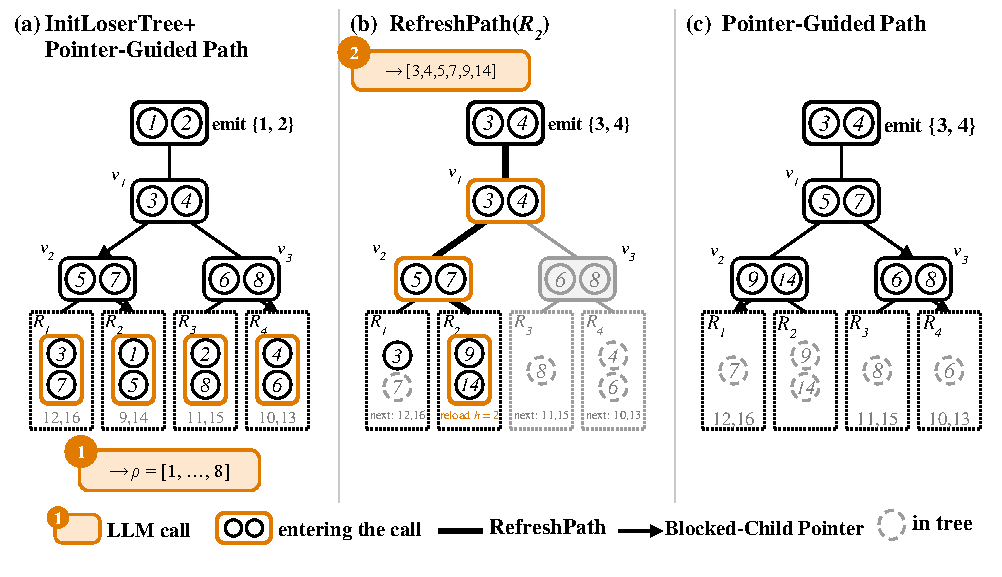
\includegraphics[width=0.95\linewidth]{fig/segment_loser_tree_exp.pdf}
    \caption{Segmented loser tree ($m  = 8 \Rightarrow d =2, h = 2$) }
    \label{fig:eg:segment_loser_tree}
\end{figure}

\begin{example}\label{ex:alg3seg}
Fig.~\ref{fig:eg:segment_loser_tree} illustrates a segmented loser tree with fan-in $k = 4$ and a listwise batch size $m = 8$. 
Thus, the tree depth $d=\max(1,\lceil\log_2 4\rceil)=2$ and the segment length $h=\lfloor 8/(1+2)\rfloor=2$. 
In Fig.~\ref{fig:eg:segment_loser_tree}(a), each leaf, $R_1$, $R_2$, $R_3$, and $R_4$, load two head items, 
These eight items are ranked by one listwise call, and the tree is initialized by bottom-up tournaments where two loser items are retained in each node. The blocked-child pointers identify when the winner $[1, 2]$ is emitted, either left or right subtree will be refreshed. For node $v_2$ with loser $[5, 7]$, a two-way merge of its children $R_1, R_2$ will first exhaust the items $[1,5]$ because of the local order $[1, 5, 3, 7]$. $R_1$ is non-exhausted due to 7 falling behind $5$. Therefore, the pointer of $v_2$ points to the leaf with $R_2$. Similarly, the internal node $v_1$ points its child $v_2$. That is because at node $v_1$, winner $[1, 3]$ from $v_2$ competes with winner $[2, 4]$ from $v_1$, and the merge result $[1, 2, 3, 4]$ making $v_2$ earlier exhausts its winner. From the perspective of two-way merge, the pointer identifies which child provide a safe prefix, and temporary blocks refreshing on the other child. 
After the winner $[1, 2]$ emits, the affect path $(v_1, v_2, R_2)$ is identified. Two items are refilled into $R_2$ and a listwise call is used to refresh this path as shown in Fig.~\ref{fig:eg:segment_loser_tree}(b). 

% In Fig.~\ref{fig:eg:segment_loser_tree}(a), the four initial leaf segments $R_1$, $R_2$, $R_3$, and $R_4$ contain the first two items of their runs. \textsc{InitLoserTree} ranks these eight items in one listwise call, constructs the tree from the resulting rank map, and certifies the root prefix $[1,2,3]$. Before any item is emitted, the left-child segment $[1,3]$ competes with the right- child segment $[2,4]$ at the root. In their merged order $[1,2,3,4]$, the left segment is exhausted after contributing $3$, while the right segment still retains $4$. The root therefore records the left child as blocked and retains $4$ until the left child is replenished. The same reasoning applies at the left internal node, recording $R_2$ as its blocked child. Following these records from the root therefore determines the unique refresh path from the root through the left internal node to $R_2$. Since $h=2$ and unread items remain, the root emits the complete segment $[1,2]$ but retains $3$ for the next refresh. As shown in Fig.~\ref{fig:eg:segment_loser_tree}(b), \textsc{RefreshPath} reloads $[9,14]$ from $R_2$ and ranks it together with the retained segment $[5,7]$ and the root items $[3,4]$. The resulting refresh window is $[3,4,5,7,9,14]$. Replaying this order along the path makes $[3,4]$ the next root segment. 
% repeats the merge of Figure~3 with the segmented tree and
% $m=8$. Fan-in $k=4$ gives depth $d=\max(1,\lceil\log_2 4\rceil)=2$
% and segment length $h=\lfloor 8/(1+2)\rfloor=2$, so every leaf
% initially holds two items of its run. Windowed initialization ranks
% the $gh=8$ leaf-resident items in $\lceil gh/m\rceil=1$ call, giving
% $\rho=[1,\dots,8]$; the tree is then built by lookups: $\{1,3\}$
% ascends past $\{5,7\}$, $\{2,4\}$ past $\{6,8\}$, and the root
% receives and emits $\{1,2\}$, with $\{3,4\}$ stored as the root's
% loser segment. \textsc{RefreshPath}$(R_2)$ reloads leaf~2 with the
% next $h=2$ items $\{9,14\}$ and ranks the $(1+d)h=6$-item window
% $[3,4,5,7,9,14]$ with one call. Balanced halving replays the path:
% the pool $\{9,14\}$ loses to the stored segment $\{5,7\}$, which
% ascends and in turn loses to $\{3,4\}$; each node keeps the bottom
% half as its new loser, and the root emits $\{3,4\}$. One call
% therefore ranks six items and emits $h=2$, against three ranked and
% one emitted per call in Figure~3.
\end{example}

\section{Token Cost Model}
\label{sec:cost}

We derive token cost models w.r.t. fan-in $k$ in sliding-window, loser-tree, and segmented loser-tree merge algorithms.
We use the number of listwise calls during the merge phase (Phase 2 of Algorithm~\ref{alg:semantic_external_merge}) as a linear proxy of total token cost. Under a fixed prompt template, a fixed batch size $m$, and expected item serialization length, each listwise call consumes a similar amount of input and output tokens.

Let $a \in \{\SD,\LT,\SLT\}$ denote a merge algorithm with sliding window (\SD), loser tree (\LT), or segmented loser tree (\SLT). The cost model $\Cost_a(k;n,m)$ measures the number of listwise calls regarding the fan-in $k$, given the item number $n$ and batch size $m$. The optimal $k$ that minimizes token cost can be derived from
\begin{align}
    k^{\star}_{a}
    =\arg\min_{k\in\mathcal{K}_a}
      \Cost_{a}(k;n,m).
    \label{eq:merge-cost-model}
\end{align}
where $\mathcal{K}_a$ is the feasible fan-in range of algorithm $a$. We assume $n>m$ and $m\ge4$ without loss of generality.

\begin{proposition}[$k$-way Merge Token Cost]
Let $\Pass_a(k)$ denote the number of merge passes for algorithm $a$ under fan-in $k$, and let $\Pcost_a(t,k;n,m)$ denote the per-pass token cost of algorithm $a$ at the $t$-th merge pass. The total merge-stage token cost is
\begin{align}
    \Cost_a(k;n,m)
    &=\sum_{t=0}^{\Pass_a(k)-1}
      \Pcost_a(t,k;n,m),
      \label{eq:total-merge-cost}\\
    \Pass_a(k)
    &=\left\lceil
      \log_k\left\lceil\frac{n}{m}\right\rceil
      \right\rceil,
      \qquad a\in\{\SD,\LT,\SLT\}.
      \label{eq:number_merge_pass}
\end{align}
\end{proposition}
It is worth noting that, as shown in Eq.~\eqref{eq:number_merge_pass}, for the same fan-in $k$, the three algorithms have the same number of merge passes in Phase 2 (Algorithm~\ref{alg:semantic_external_merge}). Therefore, their cost differences come from the per-pass term $\Pcost_a(t,k;n,m)$, which captures the patterns of how each algorithm uses listwise calls inside one pass.
We next derive $\Pcost_a(t,k;n,m)$ for each algorithm.
Complete derivations and corner cases are provided in our technical report~\cite{appendix2027} (Appendix~\ref{sec:cost-derivations}).
We use $r_0=\lceil n/m\rceil$ and $r_t=\lceil r_0/k^t\rceil$ to denote the number of runs at the beginning and the $t$-th merge pass, respectively. 
At merge pass $t$, $G_t = \lceil r_t/k\rceil$ denotes the number of groups, and each group contains $n_t= mk^t$ items to rank where $n_0 = m$.
We assume that in each pass, the sorted runs are of balanced length. 


\stitle{Per-pass token cost for sliding window.}
Here we derive the cost model in the average case, where items from sorted runs are uniformly interleaved in the result permutation $\Pi$. This condition is suitable when runs are generated by balanced partitioning, making the expected safe prefix length, $\mu_{\SD}(k,m)$, easy to derive.
For sliding window merge, the feasible fan-ins are $\mathcal K_{\SD}=\{2,\ldots,\lfloor m/2\rfloor\}$.
%, where the upper bound ensures that each active run contributes at least two items to a full window.

\begin{theorem}[$\Pcost_{\SD}$ for sliding window]
Let $h_k=\lfloor m/k\rfloor$ be the per-run ranking quota for fan-in $k$, $b_k=kh_k\le m$ be the actual batch size, and $\mu_{\SD}(k,m)$ be the expected safe prefix length of a listwise call. The per-pass token cost at the $t$-th merge pass is
\begin{align}
    \Pcost_{\SD}(t,k; n,m)
    &=\sum_{t = 1}^{G_t}
      \frac{n_{t}}
           {\mu_{\SD}(k,m)} =\frac{n}{\mu_{\SD}(k,m)},
      \label{eq:pcost-sw}\\
    \mu_{\SD}(k,m)
    &=(b_k+1)\prod_{\ell=1}^{k}
      \frac{\ell h_k}{\ell h_k+1}.
      \label{eq:mu-sw}
\end{align}
\end{theorem}
\begin{proof}[Proof Sketch:]
Under uniform random interleaving, the maximum $M_i$ among run~$i$'s $h_k$ items satisfies $\Pr(M_i\le x)=x^{h_k}$. Thus, for the first-exhaustion threshold $\tau=\min_i M_i$, $\Pr(\tau>x)=(1-x^{h_k})^k$. Order-statistic calibration gives
$\mathbb{E}[Y]=(b_k+1)\int_0^1\Pr(\tau>x)\,dx
=(b_k+1)\prod_{\ell=1}^{k}\frac{\ell h_k}{\ell h_k+1}
=\mu_{\SD}(k,m)$.
A group $j$ therefore requires
$n_{t}/\mu_{\SD}(k,m)$ expected calls. Summing over the non-singleton groups proves the formula.
\end{proof}

% \etitle{Fan-in selection.}
% The sliding-window cost model is a finite discrete optimization over $k\in\mathcal K_{\SD}$. We therefore evaluate $\Cost_{\SD}(k;n,m)$ for every feasible integer fan-in and select the minimizer.



\stitle{Per-round token cost for loser tree.} 
\label{subsec:cost-loser-tree}
In merge pass $t$, considering a group with $n_t$ items to rank, the token cost to merge this group by \textsc{MergeGroup} consists of two parts: first, two-way sliding window merge for loser tree construction. If $k < m$, this part is reduced to one listwise. Otherwise, it contains $\lceil {k}/{m}\rceil$ Phase 1 listwise, together with the total cost of Phase 2 listwise of sliding window to process $k$ representatives, i.e., $\mathcal K_{\LT}=\{2,\ldots,\min(r_0,2^{m-1})\}$.
Second, for path refresh, $n_t$ listwise calls process these $n_t$ items.
\begin{proposition}[$\Pcost_{\LT}$ for loser tree]
The per-round token cost at the $t$-th merge pass for loser tree merge is
\begin{align}
    \Pcost_{\LT}(t,k;n,m)
    &=\sum_{t = 1}^{G_t}
      \left(
        n_{t}
        +\Cost_{\SD}(2, k, m) + \left\lceil \frac{k}{m} \right\rceil
      \right) \nonumber\\
    &= n + {G_t} \left( \Cost_{\SD}(2, k, m) + \left\lceil \frac{k}{m} \right\rceil \right). 
    \label{eq:pcost-lt}
\end{align}
\end{proposition}


% \begin{proof}[Proof Sketch:]
% Each emitted item refreshes the winning root path with one call, yielding the $n_{t,j}$-call refresh term for group $j$. Loser tree $j$ first ranks $q_{t,j}=\lceil k_{t,j}/m\rceil$ chunks and then merges them according to $\mathcal T_{q_{t,j}}$; by Eq.~\eqref{eq:init-sw}, this costs $\mathrm{Init}_{\SD}(k_{t,j},m)$. Summing the disjoint refresh and initialization costs over the non-singleton groups proves the formula.
% \end{proof}
Recall that for loser tree merge, in one pass, $\textsc{RefreshPath}$ emits all $n$ items exactly once, and each emission issues one listwise. $\textsc{InitLoserTree}$ ranks only $r_t= \lceil n/(mk^t)\rceil$ representatives in total. The cost is dominated by the term from $\textsc{RefreshPath}$. Therefore, in practice, we use a per-round cost $\Pcost_{\LT}(t,k;n,m) =n$ to compute the total cost in Eq.~\eqref{eq:total-merge-cost} and select fan-in $k$ in $\mathcal{K}_{\LT} = \{2, \cdots, 2^{m - 1}\}$.

% For loser tree merge, the path refresh processes all items once, whereas initialization ranks only $r_t= \lceil n/(mk^t)\rceil$ representatives in total, 

% The refresh term therefore dominates the initialization term in our setting, making the number of merge passes the decisive factor. Hence, over $\mathcal K_{\LT}=\{2,\ldots,r_0\}$, the largest feasible fan-in, $k=r_0$, is selected, yielding $\Pass_{\LT}(k)=1$ and the minimum predicted cost.

\stitle{Per-round token cost for segmented loser tree.} 
For segmented loser tree, we have tree depth $d = \max(1, \lceil\log_2 k \rceil)$, and segment length $h = \lfloor {m}/({1+d})\rfloor$. Per-group merge cost is similar to that of loser tree, but there still remains two differences. 
First, for tree construction, the sliding window merge need to rank $kh$ representatives for $k$ runs.
Second, for path refresh, $\lceil n_t/h \rceil$ listwise calls process these $n_t$ items.
\begin{proposition}[$\Pcost_{\SLT}$ for segmented loser tree] The per-round token cost at the $t$-th merge pass for segmented loser tree merge is 
\begin{align}
    \Pcost_{\SLT}(t,k;n,m)
    &=\sum_{t = 1}^{G_t}
      \left(
        \left\lceil
          \frac{n_{t}}{h}
        \right\rceil
        + \Cost_{\SD}(2, kh, m) + \left\lceil \frac{kh}{m} \right\rceil
      \right) \nonumber \\
    & =  \left\lceil
          \frac{n}{h}
        \right\rceil + {G_t} \left(\Cost_{\SD}(2, kh, m) + \left\lceil \frac{kh}{m} \right\rceil \right)
    \label{eq:pcost-slt}
\end{align}
\end{proposition}


% \begin{proposition}[Proof Sketch:]
% Balanced path replay preserves a pool of $h_{t,j}$ items in loser tree $j$, so one call emits $h_{t,j}$ items and the group requires $\lceil n_{t,j}/h_{t,j}\rceil$ refreshes. Loser tree $j$ ranks its $k_{t,j}h_{t,j}$ resident items with the same smallest-first initializer, costing $\mathrm{Init}_{\SD}(k_{t,j}h_{t,j},m)$. Summing both call populations over the non-singleton groups proves the formula.
% \end{proposition}
For segmented loser tree, the path refresh term $\lceil{n}/{h}\rceil$ may no longer dominate Eq.~\eqref{eq:pcost-slt} for $h \geq 2$. We therefore preserve the cost term of tree construction by evaluating $\Cost_{\SD}(2;kh,m)$, when selecting a fan-in $k$ in $\mathcal K_{\SLT}=\{2,\ldots,\min(r_0,2^{m-1})\}$. 

%so the refresh term no longer overwhelmingly dominates the initialization term. Increasing $k$ reduces the number of merge passes but may decrease $h_{t,j}$ and increase both refresh and initialization costs. We therefore evaluate the complete objective $\Cost_{\SLT}(k;n,m)$ over the finite feasible set $\mathcal K_{\SLT}=\{2,\ldots,\min(r_0,2^{m-1})\}$ and select the best integer fan-in.





\section{Extension to \textsf{LIMIT}~$K$ with Pipeline Execution}
\label{sec:topk}
\label{sec:topk-exec}

A \LIMIT~$K$ query requires only the prefix $\Pi_K$ items, instead of the full permutation $\Pi$. 
The level-at-a-time execution of Phase 2 in Algorithm~\ref{alg:semantic_external_merge}, which materializes every intermediate run in a merge pass before the next pass begins, is therefore necessary for \LIMIT~$K$ query. 
To efficiently support \LIMIT~$K$, we extend the physical execution of Phase 2 with a demand-driven version of the same logical merge plan, while keeping Phase 1. Specifically, the physical plan is represented as a $k$-way merge tree in which nodes are asynchronous \emph{producers}. Leaf producers scan the sorted runs generated in Phase 1, and each internal producer implements \textsc{Next}$(c)$, which returns up to $c$ items from that node's children. An internal node pulls from its children only when its local merge state requires refilling, and the root is drained until $K$ items have been produced or until the input is exhausted. We present the complete algorithm in our technical report~\cite{appendix2027}. 

The producer formulation preserves the group merge algorithms in \cref{sec:sw} and \cref{sec:lt}. A sliding window producer maintains the same candidate window as Algorithm \ref{alg:sliding_window_kway_group_merge}: it ranks the current window, emits only the safe prefix, and retains the unsafe suffix for the next round. The only difference is that refills are obtained by invoking \textsc{Next}$(c)$ on the corresponding child producers. Similarly, a loser tree producer maintains one representative per child. After emitting the winner from the root, the producer requests one new item from the winning child and refreshes only the affected leaf-to-root path, following Algorithm~\ref{alg:loser_tree_kway_group_merge}. The segmented loser tree producer adopts the same idea at segment granularity: it pulls new segments from children, refreshes the selected path, and emits the root segment. 


To implement pipeline parallelism, in the merge tree, every non-root producer is driven by a thread with a bounded queue allowing one-item lookahead. 
This allows a child producer to prepare its next output while its parent is blocked on a listwise call, enabling pipeline parallelism across adjacent merge levels and among sibling subtrees. Meanwhile, the bounded queue avoids materializing an entire intermediate level. Once the root has produced $K$ items, the executor closes the root producer and its successor producers recursively. 
Given a merge tree and a listwise ranker, each producer emits the same sequence to their counterparts that materialize intermediate groups for full ranking. That is because the differences only lie in how input items arrive. 
Therefore, execution termination after $K$ items output is lossless relative to the full ranking algorithms. 
The token cost model in \cref{sec:cost} is not applicable for \LIMIT~$K$ query. Unlike full ranking, the number of listwise calls in the pipelined algorithms for \LIMIT~$K$ is highly sensitive to the item distribution. We leave principled token cost analysis for \LIMIT~$K$ as future work.
% full-ranking schedule materializes every intermediate run before the next
% merge pass starts.  We therefore retain Phase~1 and the fan-in chosen by
% the full-ranking cost model, but change the execution form of Phase~2.
% The same merge schedule is represented as a tree of asynchronous
% \emph{producers}: leaves serve the pre-sorted Phase-1 runs, and each
% internal node exposes \textsc{Next}$(c)$, which returns up to $c$ items
% from that node's merged order.  A node pulls from its children only when
% its local merge state needs refilling, and the root is drained for exactly
% $K$ items.  The complete procedures are given in
% Appendix~\ref{sec:topk-pseudocode}.

% This transformation does not change the group mergers themselves.  A
% sliding-window producer maintains the same sticky candidate window,
% ranks it, emits only the certified prefix, and keeps the uncertified
% suffix for the next round; refills are obtained by pulling the relevant
% children instead of advancing materialized-run cursors.  A binary
% loser-tree producer initializes from one head per child, emits the root
% winner, pulls one replacement from the winning child, and refreshes only
% that leaf-to-root path.  The segmented variant applies the same
% replacement to segment refills and continues to emit the root segment
% produced by a path refresh.

% Every non-root merge producer is advanced by a background task through a
% bounded queue with one-item look-ahead.  Consequently, a child can prepare
% its next item while its parent is waiting for a listwise call, allowing
% adjacent merge levels and sibling subtrees to overlap without
% materializing an entire level.  The one-item bound limits speculative
% work.  Once the root has returned $K$ items, the executor closes it and
% recursively cancels the outstanding producer tasks.




% For a fixed grouping and deterministic listwise ranker, each producer
% emits the same sequence as its materialized group merger because it uses
% the same state transitions and differs only in how input items arrive.
% Moreover, if an item ranks below the first $K$ positions within any
% producer subtree, at least $K$ items from that same subtree precede it, so
% it cannot belong to the global top $K$.  Capping every producer at $K$
% items and stopping the root after $K$ outputs are therefore lossless.
% The experiments in \cref{sec:exp:topk} show that this demand-driven
% execution substantially reduces tokens and latency while preserving
% top-$K$ quality.

% Approved concept trial: PR7 cursor/recovery-limit-ondemand-trial-a880 (viz/recovery/limit)
\begin{figure*}[t]
  \centering
  \includegraphics[width=\textwidth]{limit-ondemand.pdf}
  \caption{\textbf{Optional concept trial (not final).}
  Demand-driven LIMIT on the shared 16-element runs, $K{=}2$.
  Not a measured result and not an execution trace.
  The downstream drain holds \emph{emitted}.
  A dashed arrow is one request downward; a solid arrow is one yield upward.
  In (c), \emph{emitted}${=}K$, so the next request is not issued, and the hollow items stay in the runs.
  The gray dotted arrow is \texttt{finally} \texttt{aclose}, drawn as cleanup.
  Full is a separate execution mode, not $K{=}\infty$.
  The user has not yet decided whether to keep this figure in the camera-ready paper.}
  \label{fig:limit-demand-trial}
\end{figure*}


